\documentclass[a4paper, 12pt]{article}
\usepackage[T1]{fontenc}
\usepackage{lmodern}
\usepackage{color}
\usepackage{amsfonts}
\usepackage{epstopdf}
\usepackage{matlab}
%\documentclass{book}
\usepackage{blindtext}
\usepackage{hyperref}
\usepackage[brazil]{babel}
\usepackage{amssymb}
\usepackage[utf8]{inputenc}
\usepackage{amsmath}
\usepackage{indentfirst}
\usepackage{graphicx}
\usepackage{multicol,lipsum}
\usepackage[a4paper,
top=3cm, left=3cm, bottom=3cm, right=3cm]{geometry}
\usepackage{setspace}
\usepackage{multirow}
\usepackage{float}
\usepackage[dvipsnames]{xcolor}
\usepackage[table]{xcolor}
%\usepackage{pdflscape}
\usepackage[DIV=15]{typearea}
\usepackage[nottoc]{tocbibind}
\usepackage[sort,numbers]{natbib}
%\usepackage{cite}
\usepackage{matlab}


\documentclass[letterpaper]{article}
% bib pack %%%%%%%%%%%%%%%%%%%%%%%%%%%%%%%%%%%%%%%%%%%%%%%%%%%%%%%%%%%%%%%%%%%%%
\usepackage[utf8]{inputenc}
\usepackage{geometry}
    \geometry{left=3cm,right=2cm,top=2cm,bottom=2cm}
%
\usepackage[spanish]{babel}
%
\usepackage[fixlanguage]{babelbib}
    \bibliographystyle{babunsrt}
%
\usepackage{url}

\begin{document}
%\maketitle

\begin{titlepage}
	\begin{center}
		

\vspace{10pt}
%\begin{figure}[H][!ht]
%\centering
%
\includegraphics{puc-rio-logo.png}

%\end{figure}
\begin{figure}[!ht]
\centering

\includegraphics{images/puc-rio-logo.png}
\end{figure}
\huge{Laboratório de Controles e Servomecanismos}
        \vspace{70pt}
        
		\textbf{ENG1418}
		\textbf{\large{\\ }}
		
		\vspace{30pt}
		\textbf{\small{\\Trabalho 8}}
		\vspace{75pt}
		
	\end{center}
	
	\begin{flushleft}
		\begin{tabbing}
			Aluno(a)\qquad\qquad\=\>Iury Saboia Martins 1620675 \\ \>Paloma Fernanda Loureiro Sette - 1621595\\
			
			Professor(a)\>Vivian Suzano Medeiros\\
	\end{tabbing}
		  
	\end{flushleft}
	\begin{center}
		%\vspace{\fill}
		\vspace{90pt}
		Rio de Janeiro, 07 de Julho de 2022
	\end{center}
\end{titlepage}
%%%%%%%%%%%%%%%%%%%%%%%%%%%%%%%%%%%%%%%%%%%%%%%%%%%%%%%%%%%
\newpage
\tableofcontents
\thispagestyle{empty}

\newpage
\pagenumbering{arabic}

\newpage

%\newcommand{\listequationsname}{Lista de Equações}
%\newlistof{myequations}{equ}{\listequationsname}
%\newcommand{\myequations}[1]{%
%\addcontentsline{equ}{myequations}{\protect\numberline{\theequation}#1}\par}

%\listofmyequations
\newpage


\newpage

\listoffigures
\thispagestyle{empty}

\newpage
%%%%%%%%%%%%%%%%%%%%%%%%%%%%%%%%%%%%%%%%%%%%%%%%%%%%%%%%%
%%%%%%%%%%%%%%%%%%%%%%%%%%%%%%%%%%%%%%%%%%%%%%%%%%%

\newpage

\thispagestyle{empty}

\newpage

\section{Introdução}
Dispositivos de simulação de paraquedismo são cada vez mais comuns tanto para entretenimento quanto para treinamento de paraquedismo. Para tal atividade, o dispositivo que sopra o ar e mantém a pessoa estável em uma determinada altura deve ser extremamente confiável.

Neste sentido, o estudo deste tipo de equipamento é desafiador, pois utiliza princípios como arrasto
aerodinâmico e comportamento de escoamento de fluidos, além de um sistema eletromecânico de
acionamento.

\section{Abordagem}
Observe a figura esquemática do sistema, abaixo:

\begin{figure}[H]
\centering
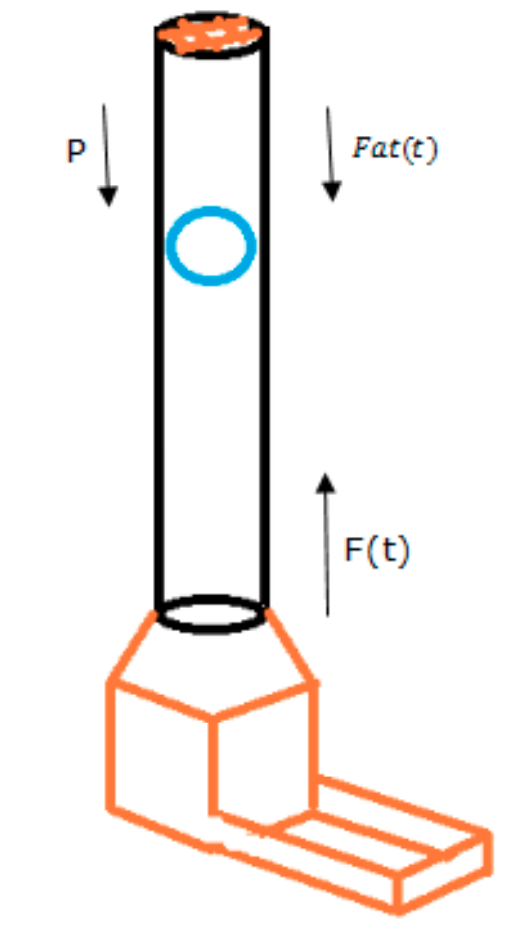
\includegraphics[scale = 0.5]{images/esquematico.png}
\label{filtro1}
\caption{Esquemático do sistema}
\end{figure}

Podem ser escritas as seguintes equações:
\begin{equation}
    \begin{cases}
    \dot{x}\ =v(t) \\
    m\ddot{x}\ =-mg-Fat(t)+F(t)
    
    \end{cases}
\end{equation}

Este sistema pode ser representado na seguinte forma em espaço-estado:

\begin{equation}
    \left[\begin{matrix}0&1\\0&-k_1v\left(t\right)+F\left(t\right)\\\end{matrix}\right]X+\left[\begin{matrix}0\\1/m\\\end{matrix}\right]
\end{equation}

\begin{equation}
Y=\left[\begin{matrix}1&0\end{matrix}\right]X
\end{equation}

Sendo a entrada a força de propulsão do ventilador e a saída a posição vertical da bolinha. Passando
para função de transferência, se tem:

\begin{equation}
    P(s)=\frac{1/m}{s(s+k_{1}/m)}
\end{equation}

\subsection{Parte 1 - Simulações com o MATLAB®}
Consideremos o sistema de controle apresentado no sistema a seguir:

\begin{figure}[H]
\centering
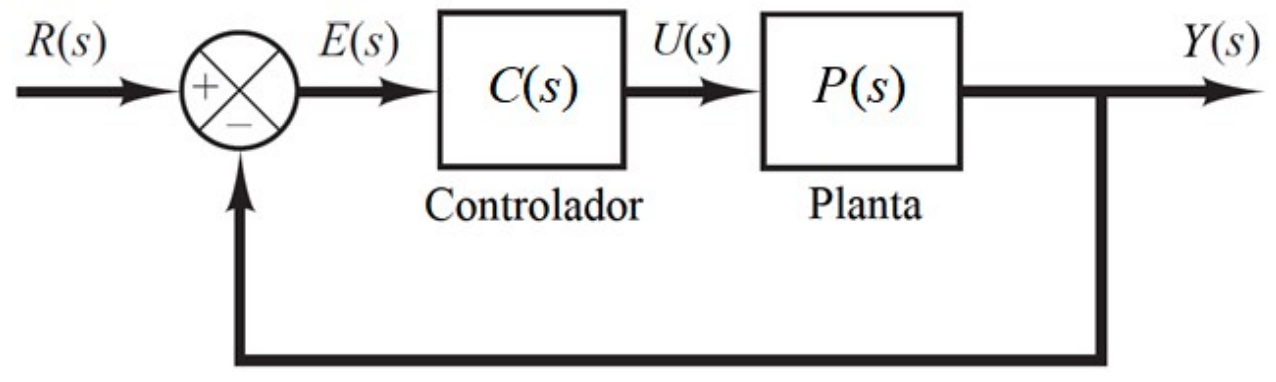
\includegraphics[scale = 0.5]{images/diagrama-bloco.png}
\label{filtro1}
\caption{Sistema de controle}
\end{figure}

Onde $P(s)$ é a função de transferência do soprador, apresentada anteriormente e $C(s)$ é a função de
transferência do controlador. Considere que a massa da bolinha é $2.7$ gramas e o coeficiente de arrasto
aerodinâmico $k_{1}$ é $0.036 kg/s$. Para o sistema em malha fechada, considere que o sinal de entrada de referência é um degrau de amplitude $10 cm$.

\subsubsection{Parte (i)}
Devemos simular o sistema sem controle, ou seja, somente a planta $P(s)$, para uma entrada degrau unitário, analisando o comportamento encontrado.

Segue abaixo o código produzido no  MATLAB®:

\sloppy
\epstopdfsetup{outdir=./}
\graphicspath{ {mathgraphics} }

\matlabheadingtwo{\color{blue}{Questão 1 - Parte (i)}}

\begin{matlabcode}
clc; clear all; close all;

%inicializando os parametros
s = tf('s');

%Parametros dados
m = 0.0027; %massa em kg;
k1 = 0.036; %coeficiente de atrito = 0.036kg/s
R = 0.1; %step input (m) R = 10cm = 0.1m

%Função de transferência da planta
P = (1/m)/(s(s+k1/m))
\end{matlabcode}
\begin{matlaboutput}
P =
 
      370.4
  -------------
  s^2 + 13.33 s
 
Continuous-time transfer function.
\end{matlaboutput}
\begin{matlabcode}

%Plotando a resposta ao degrau
figure(1)
step(P,opt);
\end{matlabcode}

A resposta ao degrau do sistema do sistema é mostrada abaixo. Podemos observar claramente que a saída está aumentando com o tempo e, portanto, não é limitada para uma entrada limitada.

Portanto, o sistema em malha aberta (sem controle) NÃO É BIBO-ESTÁVEL. Já o sistema realimentado, converge, ou seja, tem 2 polos no SPAE.



\begin{center}
\begin{figure}[H]
\centering
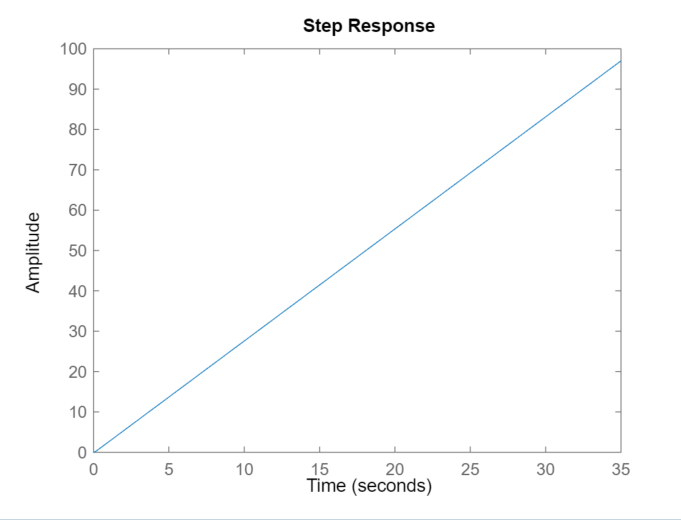
\includegraphics[scale = 1.2]{images/step-responde_line.png}
\caption{Resposta ao degrau}
\end{figure}\end{center}
\begin{matlabcode}

opt = stepDataOptions('StepAmplitude',R);
sys = feedback(P, 1)
\end{matlabcode}
\begin{matlaboutput}
sys =
 
          370.4
  ---------------------
  s^2 + 13.33 s + 370.4
 
Continuous-time transfer function.
\end{matlaboutput}
\begin{matlabcode}
step(sys,opt)
\end{matlabcode}
\begin{center}
\begin{figure}[H]
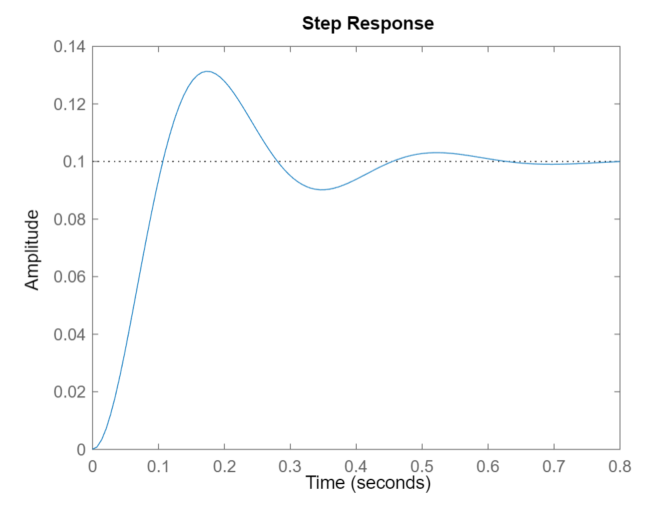
\includegraphics[scale = 1.2]{images/step-response_feedback.png}
\caption{Feedback 1.1}
\end{figure}\end{center}


\newpage
\subsubsection{Parte (ii)}
Neste item, devemos considerar, inicialmente um \textbf{controlador proporcional}. Devemos fazer a \textbf{função de transferência em malha fechada} em função do ganho $K_p$. 

\begin{equation}
    \frac{Y(s)}{R(s)} = \frac{C(s)P(s)}{1+C(s)P(s)}
\end{equation}

Substituindo P(s) e C(s) na equação, teremos:

\begin{equation}
    \frac{Y(s)}{R(s)} = \frac{370.4K_p}{s^2+13.33s+370.4K_p}
\end{equation}

Podemos ver que \textbf{o sistema de malha fechada acima é um sistema de segunda ordem}. Cujo os \textbf{polos} são dados por:

\begin{equation}
    -\xi\omega_n \pm j\omega_n\sqrt{1-\xi^2}
\end{equation}

Comparando a equação característica com o sistema geral de segunda ordem, obtemos:

\paragraph{Frequência Natural}
\begin{equation}
    \omega_n^2=370.4K_p
\end{equation}
\begin{equation}
    \omega_n=\sqrt{370.4K_p}
\end{equation}

\paragraph{Fator de amortecimento}
\begin{equation}
    2\xi\omega_n=13.33
\end{equation}
\begin{equation}
    \xi=\frac{13.33}{2\sqrt{370.4K_p}}
\end{equation}

\paragraph{Tempo de assentamento} 
\begin{equation}
    t_a=\frac{4}{|-\omega_n\xi|}
\end{equation}

\paragraph{Erro em regime permanente para uma entrada degrau unitário}. 
\begin{equation}
    \lim_{s\to 0}(1-\frac{Y(s)}{R(s)})s=0
\end{equation}
%A partir dessas expressões, verifique analiticamente como o ganho Kp afeta o comportamento do sistema.


\subsubsection{Parte (iii)}
Neste item, devemos \textbf{simular o  sistema em malha fechada para um controlador P}. Varie o ganho proporcional $K_p$ e verificar como ele afeta o comportamento do sistema em malha fechada.

\sloppy
\epstopdfsetup{outdir=./}
\graphicspath{ {./lista8_lab_servomec_images/} }

\matlabheadingtwo{\color{blue}{Questão 1 - Parte (iii)}}

\begin{matlabcode}
kp = [0.001 0.017 0.17 1.7];
figure(1)

for k = 1:4
    sys = feedback(P*kp(k), 1);
    subplot(2,2,k)
    step(sys,opt)
    title(['Para kp = ', num2str(kp(k))])
    xlim([0 10])
end
\end{matlabcode}
\begin{center}
\begin{figure}[H]
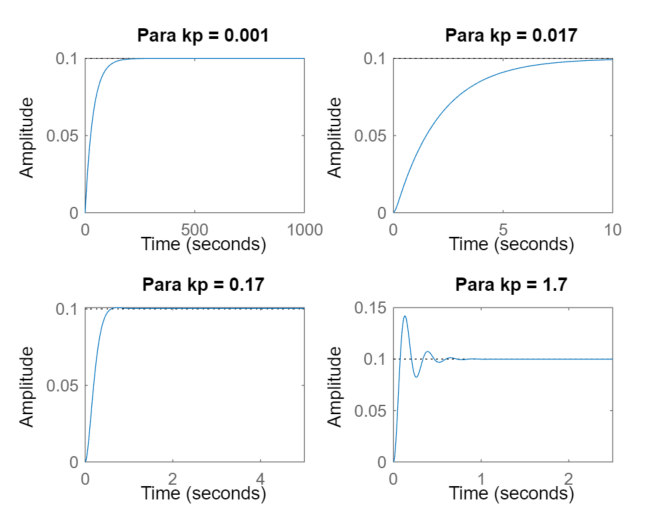
\includegraphics[scale = 1.3]{images/pt_3.png}
\caption{Resultado gráfico - Parte 1.3}
\end{figure}\end{center}

Notasse que, a medida que $K_p$ aumenta o sistema estabiliza mais rápido, em compensação, as oscilações, até o regime permanente, aumentam (maior overshoot consequentemente).

\subsubsection{Parte (iv)}
\textbf{Simularemos o sistema em malha fechada para um controlador PI}. Devemos variar os ganhos $K_p$ e $K_i$, verificando como cada um deles afeta o comportamento do sistema em malha fechada.

\sloppy
\epstopdfsetup{outdir=./}
\graphicspath{ {./lista8_lab_servomec_images/} }
 
 \matlabheadingtwo{\color{blue}{Questão 1 - Parte (iv)}}

\begin{matlabcode}
kp2 = [0 0.08 1.1 1.5];
ki = [3e-4 3e-3 3e-2 3]
\end{matlabcode}
\begin{matlaboutput}
ki = 1x4    
    0.0003    0.0030    0.0300    3.0000

\end{matlaboutput}
\begin{matlabcode}
figure(1)

for k = 1:4
    Cs = pid(kp2(k), ki(k))
    sys = feedback(P*Cs, 1);
    subplot(2,2,k)
    step(sys,opt)
    title(['Para kp = ', num2str(kp(k)) ', ki = ', num2str(ki(k))])
    xlim([0 20])
end
\end{matlabcode}
\begin{matlaboutput}
Cs =
 
        1 
  Ki * ---
        s 

  with Ki = 0.0003
 
Continuous-time I-only controller.

Cs =
 
             1 
  Kp + Ki * ---
             s 

  with Kp = 0.08, Ki = 0.003
 
Continuous-time PI controller in parallel form.

Cs =
 
             1 
  Kp + Ki * ---
             s 

  with Kp = 1.1, Ki = 0.03
 
Continuous-time PI controller in parallel form.

Cs =
 
             1 
  Kp + Ki * ---
             s 

  with Kp = 1.5, Ki = 3
 
Continuous-time PI controller in parallel form.
\end{matlaboutput}
\begin{center}
\begin{figure}[H]
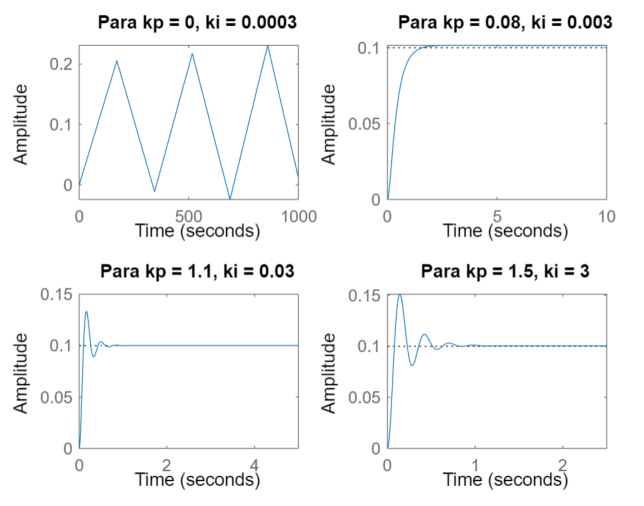
\includegraphics[scale = 1.3]{images/pt_4.png}
\caption{Resultado gráfico 1.4}
\end{figure}\end{center}

A medida que os valores de $K_i$ aumentam, as oscilações aumentam em amplitude e frequência, assim como esperado. Outro ponto importante é que, em geral, o erro em  regime permanente ainda é zero. Nota-se que há combinações de $K_p$ e $K_i$ que tornam o sistema instável.

\subsubsection{Parte (v)}
 Simularemos o sistema em malha fechada para um \textbf{controlador PD}. Varie os ganhos $K_p$ e $K_d$ e verificaremos como cada um deles afeta o comportamento do sistema em malha fechada.
 
 \sloppy
\epstopdfsetup{outdir=./}
\graphicspath{ {./lista8_lab_servomec_images/} }
 

\matlabheadingtwo{\color{blue}{Questão 1 - Parte (v)}}

\begin{matlabcode}
kp3 = [0 2.36 0.1 30];
kd = [0.01 0.0975 1 2.5]
\end{matlabcode}
\begin{matlaboutput}
kd = 1x4    
    0.0100    0.0975    1.0000    2.5000

\end{matlaboutput}
\begin{matlabcode}
figure(1)

for k = 1:4
    Cs = pid(kp3(k), kd(k))
    sys = feedback(P*Cs, 1);
    subplot(2,2,k)
    step(sys,opt)
    title(['Para kp = ', num2str(kp3(k)) ', kd = ', num2str(kd(k))])
    xlim([0 3])
end
\end{matlabcode}
\begin{matlaboutput}
Cs =
 
             
  Kp + Kd * s
             

  with Kp = 0, Kd = 0.01
 
Continuous-time PD controller in parallel form.

Cs =
 
             
  Kp + Kd * s
             

  with Kp = 2.36, Kd = 0.0975
 
Continuous-time PD controller in parallel form.

Cs =
 
             
  Kp + Kd * s
             

  with Kp = 0.1, Kd = 1
 
Continuous-time PD controller in parallel form.

Cs =
 
             
  Kp + Kd * s
             

  with Kp = 30, Kd = 2.5
 
Continuous-time PD controller in parallel form.
 
Continuous-time PD controller in parallel form.
\end{matlaboutput}
\begin{center}
\begin{figure}[H]
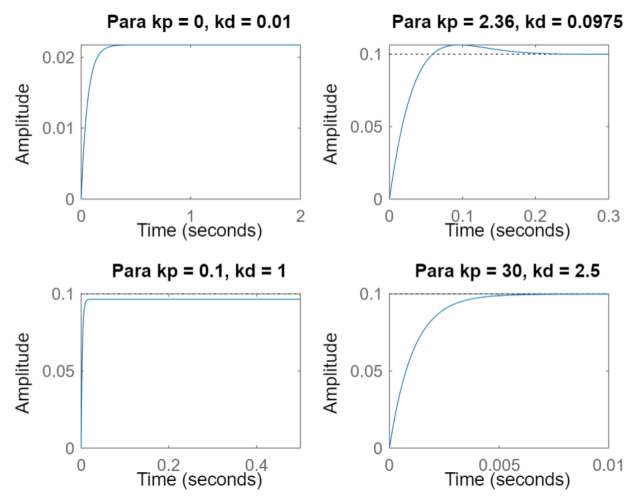
\includegraphics[scale = 1.3]{images/pt_5.png}
\caption{Resultado gráfico 1.5}
\end{figure}\end{center}

A medida que $K_d$ aumenta, o tempo para chegar ao regime permanente diminui. Em compensação, nota-se que o erro em regime permanente não é nulo em alguns casos. Dado que o sistema, realimentado, consegue chegar pos si só em regime permanete com erro zero, há combinações de $K_p$ e $K_d$ que levam o sistema a erro zero.

\subsubsection{Parte (vi)}
Simule o sistema em malha fechada para um \textbf{controlador PID}. Variaremos os ganhos $K_p$, $K_i$ e $K_d$ e verificaremos como cada um deles afeta o comportamento do sistema em malha fechada.

\sloppy
\epstopdfsetup{outdir=./}
\graphicspath{ {./lista8_lab_servomec_images/} }

\matlabheadingtwo{\color{blue}{Questão 1 - Parte (vi)}}

\begin{matlabcode}
kp4 = [0.02 0.1 0.425 1 5 20];
ki = [0.01 0.1 0.65 1 2 5] 
\end{matlabcode}
\begin{matlaboutput}
ki = 1x6    
    0.0100    0.1000    0.6500    1.0000    2.0000    5.0000

\end{matlaboutput}
\begin{matlabcode}
kd = [0.01 0.01 0.0693 0.1 0.5 2]
\end{matlabcode}
\begin{matlaboutput}
kd = 1x6    
    0.0100    0.0100    0.0693    0.1000    0.5000    2.0000

\end{matlaboutput}
\begin{matlabcode}

figure(1)

for k = 1:6
    Cs = pid(kp4(k), ki(k), kd(k))
    sys = feedback(P*Cs, 1);
    subplot(3,2,k)
    step(sys,opt)
    title(['Para kp = ', num2str(kp4(k)) ', ki = ', num2str(ki(k)) 
    ', kd = ', num2str(kd(k))])
    xlim([0 3])
    ylim([0 1.3])
end
\end{matlabcode}
\begin{matlaboutput}
Cs =
 
             1          
  Kp + Ki * --- + Kd * s
             s          

  with Kp = 0.02, Ki = 0.01, Kd = 0.01
 
Continuous-time PID controller in parallel form.

Cs =
 
             1          
  Kp + Ki * --- + Kd * s
             s          

  with Kp = 0.1, Ki = 0.1, Kd = 0.01
 
Continuous-time PID controller in parallel form.

Cs =
 
             1          
  Kp + Ki * --- + Kd * s
             s          

  with Kp = 0.425, Ki = 0.65, Kd = 0.0693
 
Continuous-time PID controller in parallel form.

Cs =
 
             1          
  Kp + Ki * --- + Kd * s
             s          

  with Kp = 1, Ki = 1, Kd = 0.1
 
Continuous-time PID controller in parallel form.

Cs =
 
             1          
  Kp + Ki * --- + Kd * s
             s          

  with Kp = 5, Ki = 2, Kd = 0.5
 
Continuous-time PID controller in parallel form.

Cs =
 
             1          
  Kp + Ki * --- + Kd * s
             s          

  with Kp = 20, Ki = 5, Kd = 2
 
Continuous-time PID controller in parallel form.
\end{matlaboutput}
\begin{center}
\begin{figure}[H]
    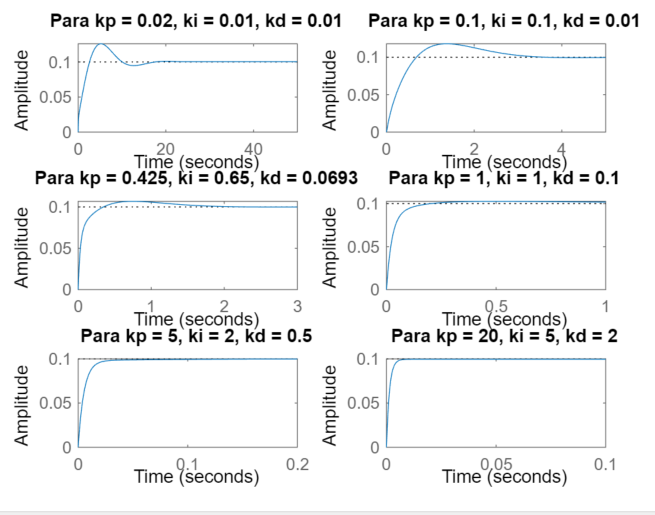
\includegraphics[scale = 1.3]{images/pt_6.png}
    \caption{Resultado gráfico 1.6}
\end{figure}\end{center}

Nota-se que o controlador PID pode combinar as caracteristicas dos diversos controladores. Assim, através de combinações entre os ganhos $K_p$, $K_d$ e $K_i$ é possível se atingir a respota desejada no sistema. Aumentando $K_i$ aumentamos um pouco as oscilações do sistema (mantendo o sistema em erro em regime permanente igual a zero), aumentando o $K_d$ diminuimos as oscilações e chegamos mais rápido ao regime permanente já, com o ganho $K_p$ insere um ganho linear no sistema fazendo com o controlador atue com uma componente linear.
\newpage

\subsection{Parte 2 - Experimento Remoto utilizando o Soprador}

\subsubsection{Parte (i)}

Utilizando o sistema em \textbf{MALHA ABERTA}, devemos inserir o seguinte conjunto de valores para velocidade e verificar quais as alturas resultantes.

Analisaremos as medições em relação a: linearidade, zona morta, atraso e outros fatores de desempenho.

\begin{center}
\begin{figure}[H]
    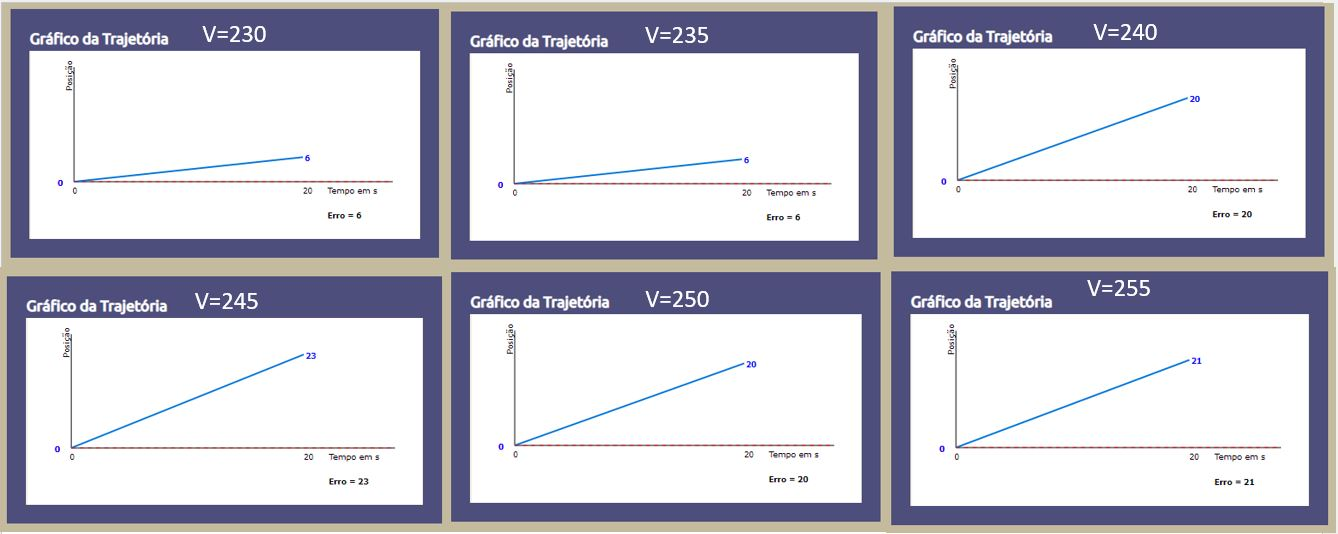
\includegraphics[scale = 0.7]{images/2_2_1.png}
    \caption{Resultado dos Soprador para  $V=[230, 235, 240, 245, 250, 255]$}
\end{figure}\end{center}

Tomando o ponto 6 como zero, o sistema possui uma zona morta para entradas entre $V=[230:235]$ em média.
A respota as entradas é, aparentemente linear.
Dado os resultados, não foi possivel avaliar se o sistema tem atraso na resposta ou não.
\subsubsection{Parte (ii)}
Repita o item anterior. As respostas foram as mesmas? Este comportamento era esperado? Por quê?\\
Os resultados em muitos teste deram similar, porêm, em alguns testes, deram diferentes. Essa diferença pode se dever a variações e erros que um sistema real pode apresentar.

\subsubsection{Parte (iii)}
Utilizando o sistema em \textbf{MALHA FECHADA}, insira o seguinte conjunto de ganhos $K_p$ e \textbf{ZERE OS DEMAIS GANHOS}. 

Altura = $15cm$. 

Analise como a variação do ganho afeta a resposta do
sistema. $Kp = [5, 8, 10, 15, 20]$.

\begin{center}
\begin{figure}[H]
    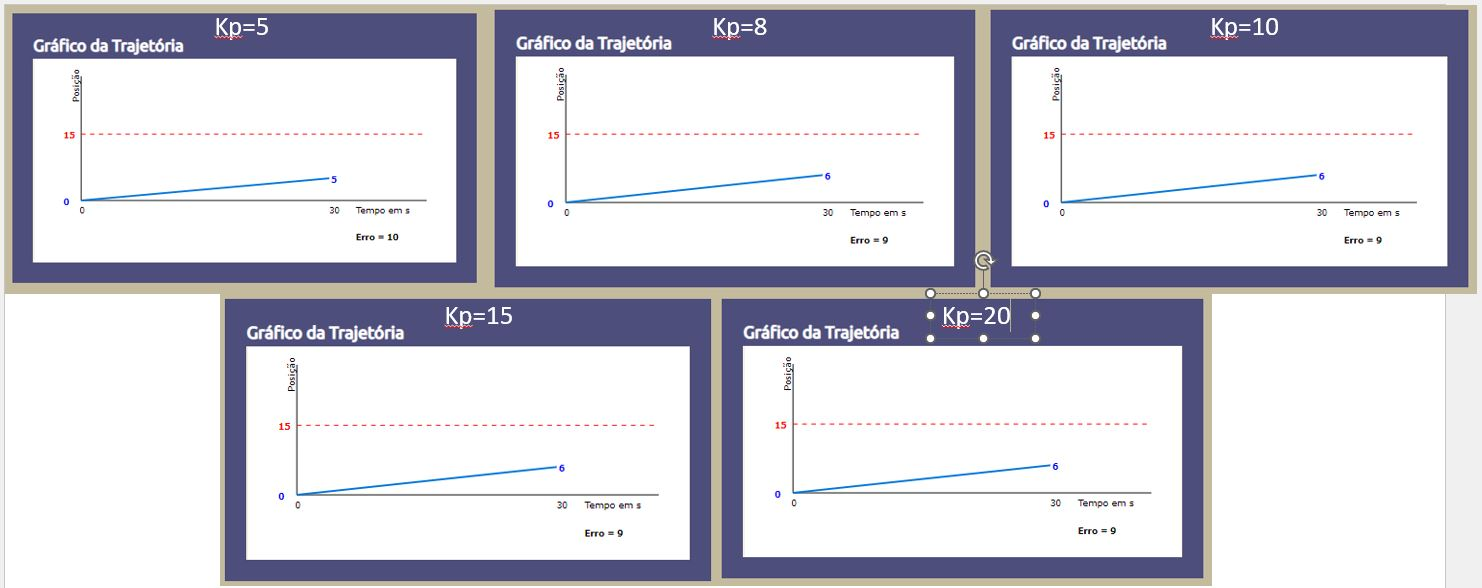
\includegraphics[scale = 0.6]{images/2.2.3.JPG}
    \caption{Resultado dos Soprador para $H=15cm$ $K_p = [5, 8, 10, 15, 20]$}
\end{figure}\end{center}

A resposta do sistema não variou com o acréscimo do ganho $K_p$. Esse resultado não era esperado dado a respota da simulação que já fora préviamente mostrada na parte anterior.

\subsubsection{Parte (iv)}
Utilizando o sistema em MALHA FECHADA, fixe $K_p$ em 10, \textbf{ZERE OS DEMAIS GANHOS} e insira o seguinte conjunto de alturas. Analise o comportamento do sistema em cada um dos casos.

\begin{center}
\begin{figure}[H]
    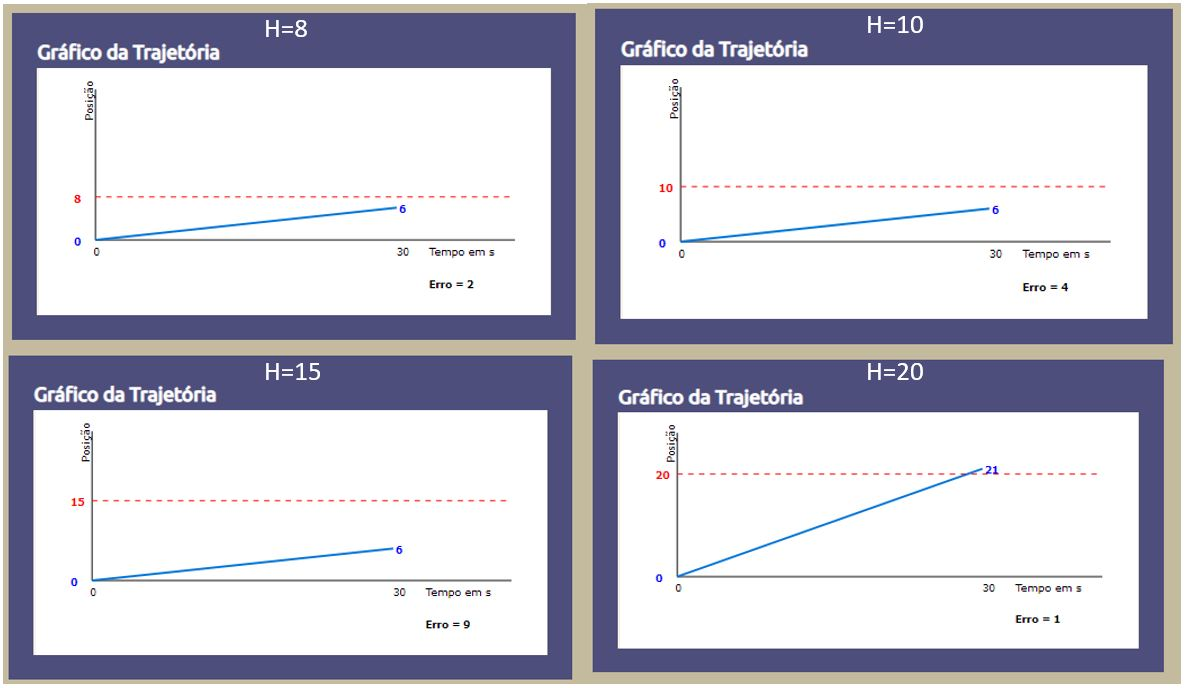
\includegraphics[scale = 0.8]{images/2.2.4.JPG}
    \caption{Resultado dos Soprador para $K_p=10$  $H = [8, 10,15, 20]$}
\end{figure}\end{center}

A resposta do sistema não variou com o acréscimo da altura de referência, salvo no ultimo teste em que foi considerado $H=20cm$.

\subsubsection{Parte (v)}
Utilizando o sistema em \textbf{MALHA FECHADA}, fixe $K_p$ em 3, ZERE $K_d$ e insira o seguinte conjunto de ganhos $K_i$. Analise como a variação do ganho afeta a resposta do sistema. \\

\begin{center}
\begin{figure}[H]
    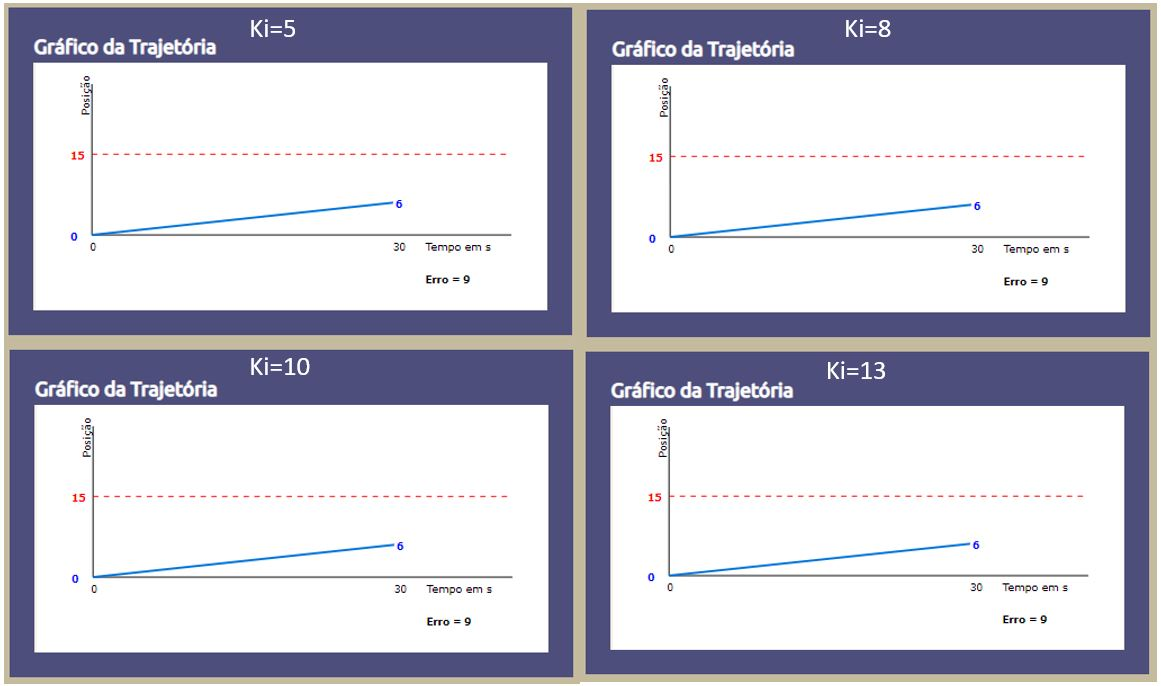
\includegraphics[scale = 0.8]{images/2.2.5.JPG}
    \caption{Resultado dos Soprador para $K_p=3$  $K_i =[5, 8, 10, 13]$}
\end{figure}\end{center}

A resposta do sistema não variou com o acréscimo do ganho $K_i$. O resultado não condiz com o esperado, o que reforça isso é que, independente do aumento do valor do ganho $K_i$ o erro da respota do sistema não zera.

\subsubsection{Parte (vi)}
Utilizando o sistema em \textbf{MALHA FECHADA}, fixe $K_p$ em 10 e $K_i$ em 8, \textbf{ZERE} $K_d$ e insira o seguinte conjunto de alturas. Analise o comportamento do sistema em cada um dos casos.\\

\begin{center}
\begin{figure}[H]
    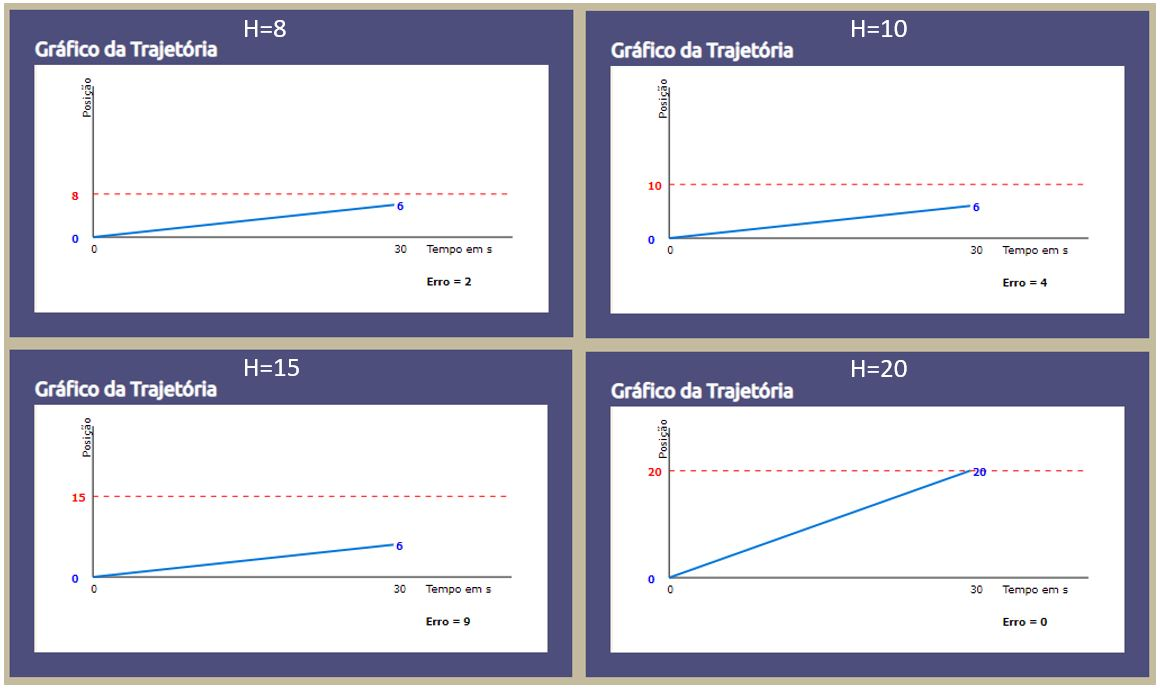
\includegraphics[scale = 0.8]{images/2.2.6.JPG}
    \caption{Resultado dos Soprador para $K_p=10$ $K_i=8$ $H = [8, 10, 15, 20]$}
\end{figure}\end{center}

Novamente a resposta do sistema só variou no ultimo teste em que foi considerado $H=20cm$.

\subsubsection{Parte (vii)}
Utilizando o sistema em \textbf{MALHA FECHADA}, fixe $K_p$ em 3, ZERE $K_i$ e insira o seguinte conjunto de ganhos $K_d$. Analise como a variação do ganho afeta a resposta do sistema. \\

\begin{center}
\begin{figure}[H]
    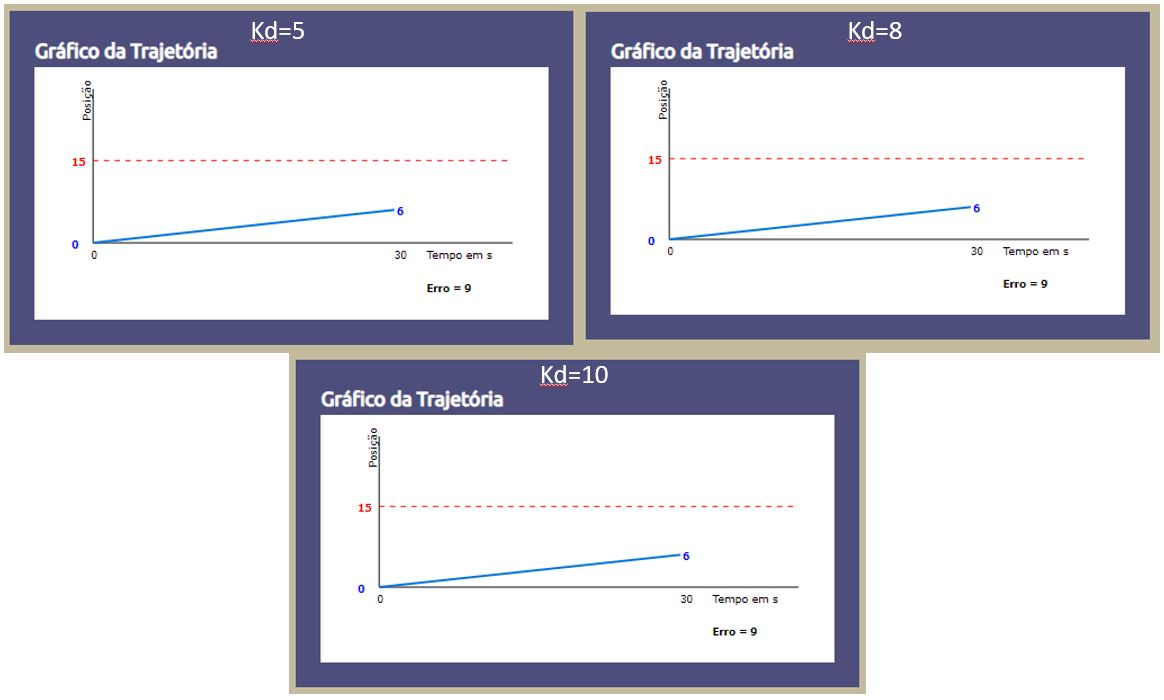
\includegraphics[scale = 0.8]{images/2.2.7.JPG}
    \caption{Resultado dos Soprador para $K_p=3$ $K_d =[5, 8, 10]$}
\end{figure}\end{center}

\subsubsection{Parte (viii)}
Utilizando o sistema em MALHA FECHADA, fixe $K_p$ em 10 e $K_d$ em 3, ZERE $K_i$ e insira o seguinte conjunto de alturas. Analise o comportamento do sistema em cada um dos casos. \\

\begin{center}
\begin{figure}[H]
    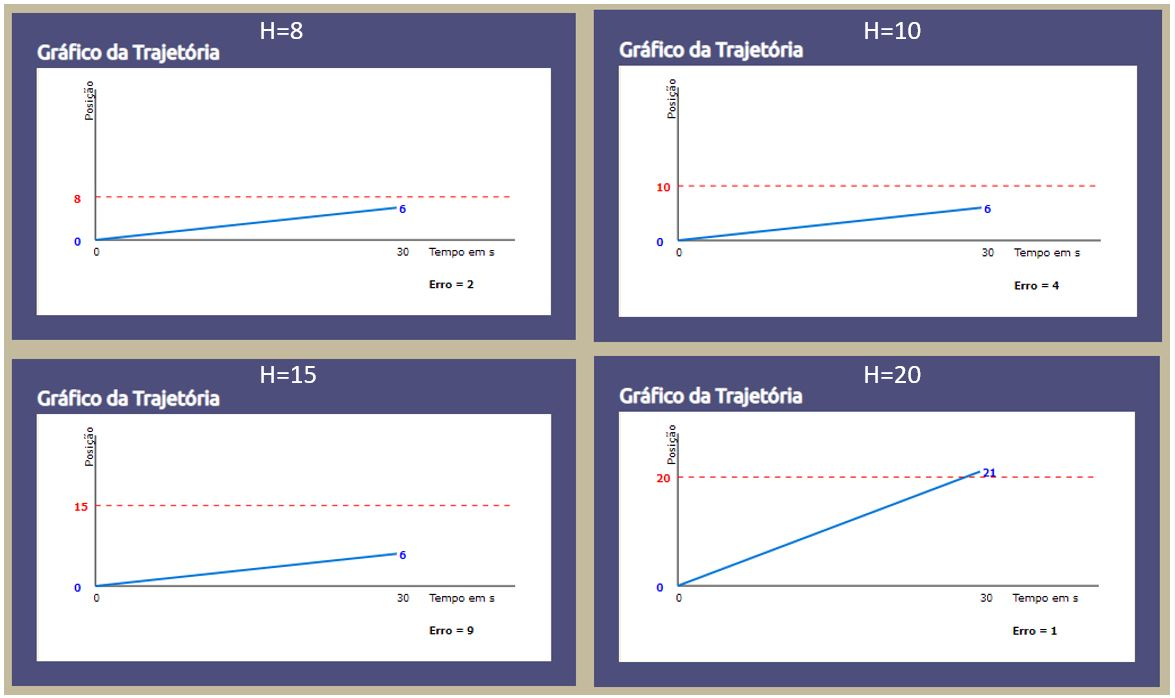
\includegraphics[scale = 0.8]{images/2.2.8.JPG}
    \caption{Resultado dos Soprador para $K_p=10$ $K_d=3$ $H = [8, 10, 15, 20]$}
\end{figure}\end{center}

A resposta do sistema não variou com o acréscimo do ganho $K_d$. Isso não é o esperado dado tal ganho deveria, ao menos, fazer com que a o tempo de chegada no regime constante se acelerasse.

\subsubsection{Parte (ix)}
 Utilizando o sistema em MALHA FECHADA, fixe $K_p$ em 10, $K_d$ em 3 e $K_i$ em 5 e insira o seguinte conjunto de alturas. Analise o comportamento do sistema em cada um dos casos.\\
 
 \begin{center}
 \begin{figure}[H]
    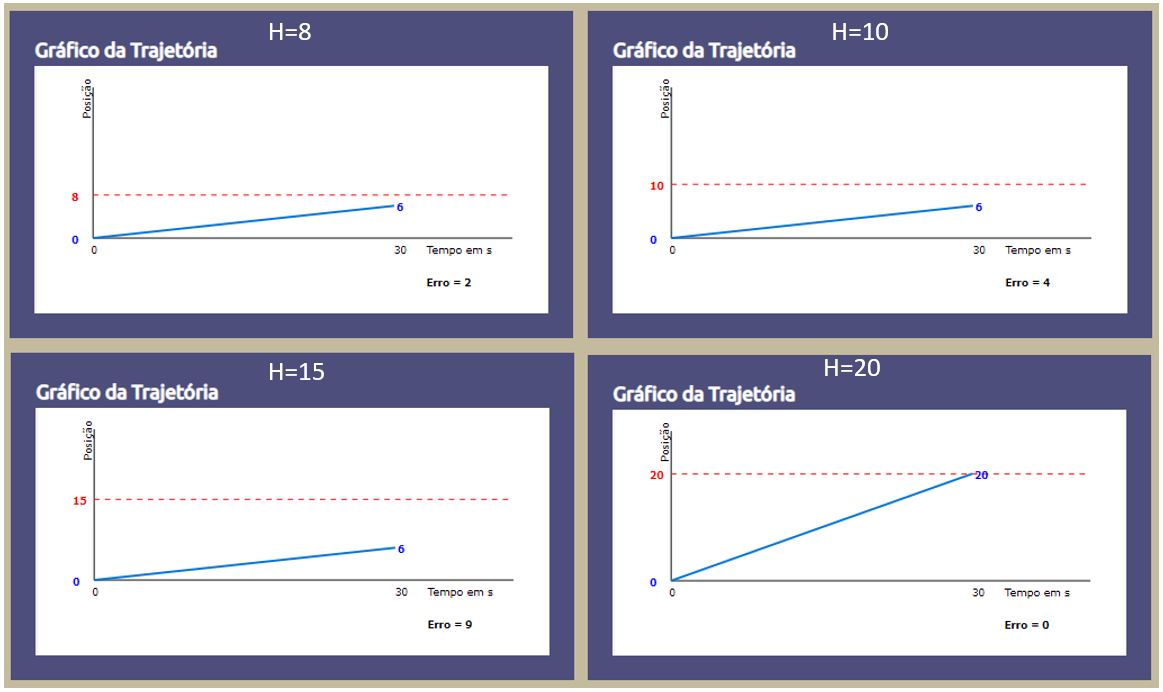
\includegraphics[scale = 0.8]{images/2.2.9.JPG}
    \caption{Resultado dos Soprador para $K_p=10$ $K_i=5$ $K_d=3$  $H = [8, 10, 15, 20]$}
\end{figure}
\end{center}
Novamente a resposta do sistema só variou no ultimo teste em que foi considerado $H=20cm$.

\newpage
% REFERENCIAS %%%%%%%%%%%%%%%%%%%%%%%%%%%%%%%%%%%%%%%%%%%%%%%%%%%%%%%%%%%%%%
    \nocite{*}
    \bibliography{src/bibliography}
    
\end{document}
\section{Referências Bibliográficas}



\end{document}